\documentclass{beamer}
\title{Xv6 Book ch1\\ Code}
\usetheme{CambridgeUS}
\usecolortheme{beaver}
\usepackage{listings}
\usepackage{kotex}
\usepackage{graphics}
\usepackage{booktabs}
\usepackage{local_dir}
\graphicspath{ {\rcufigure/xv6-book-ch1-code/}}
\author{Chang-Hui Kim}

\begin{document}

\begin{frame}
  \titlepage
\end{frame}

%% -------------------------------------------------------------------------

\section{Code: the first address space}

%% -------------------------------------------------------------------------

\begin{frame}[t, fragile]
  \frametitle{Code: the first address space}

  \begin{figure}
    \begin{lstlisting}
      // Call the entry point from the ELF header.
      // Does not return!
      entry = (void(*)(void))(elf->entry);
      entry();
    \end{lstlisting}
    \caption{in bootmain}
  \end{figure}

  \texttt{entry}
  \begin{enumerate}
  \item makes the stack pointer, \texttt{\%esp} to user stack.
  \item jumps to \texttt{main}. (main.c)
  \end{enumerate}
 
\end{frame}

%% -------------------------------------------------------------------------

\section{Code: creating the first process}

%% -------------------------------------------------------------------------

\begin{frame}[t]
  \frametitle{Code: creating the first process}
  After \texttt{main} initializes several devices and subsystems,
  it creates the first process\\

  via calling \texttt{userinit}.
  \begin{enumerate}
  \item calls \texttt{allocproc} to create proc.
  \item calls \texttt{setupkvm} to create a page table for the process. (only for kernel).
  \item calls \texttt{inituvm} to load \texttt{initcode.S}.
  \item sets up the trap frame with the initial user mode state.
  \item the stack pointer \texttt{\%esp} is set to the process's largest valied virtual
    address, \texttt{p->sz}.
  \item the instruction pointer is set to the entry point for the initcode, address 0.
  \item setting \texttt{p->state} to \texttt{RUNNABLE}.
  \end{enumerate}

\end{frame}

%% -------------------------------------------------------------------------

\begin{frame}[t]
  \frametitle{\texttt{allocproc}}

  \texttt{allocproc}
  \begin{enumerate}
  \item scans the \texttt{proc} table for a slot with state \texttt{UNUSED}.
  \item sets the state to \texttt{EMBRYO}.
  \item gives the process a unique \texttt{pid}.
  \item tries to allocate a kernel stack for the process's kernel thread.
  \end{enumerate}
  
\end{frame}

%% -------------------------------------------------------------------------

\begin{frame}[t]
  \frametitle{kernel stack}
  \begin{figure}[ht]
    \centering
    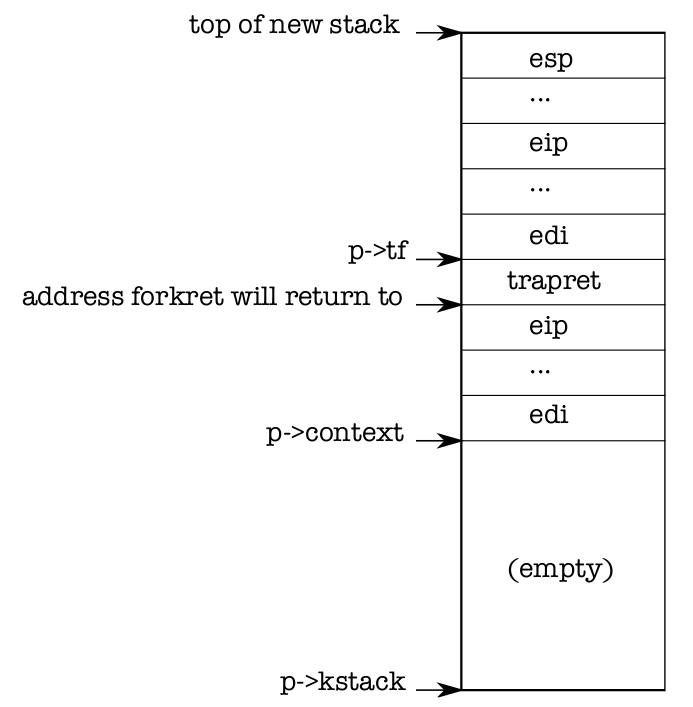
\includegraphics[width=0.6\textwidth]{fig1-4.png}
  \end{figure}

\end{frame}

%% -------------------------------------------------------------------------

\begin{frame}[t]
  \frametitle{\texttt{allocproc}}

  The context switch code sets the stack pointer to point just beyond the end of
  \texttt{p->context}.\\

  \texttt{allocproc} 
  \begin{enumerate}
  \item places \texttt{p->context} on the stack.
  \item puts a pointer to \texttt{trapret} just above it. (where \texttt{forkret} return)
  \item sets \texttt{p->context->eip} to \texttt{forkret}.
  \end{enumerate}

  Cause the kernel thread to execute at the start of \texttt{forkret}.
  
\end{frame}

%% -------------------------------------------------------------------------

\begin{frame}[t]
  \frametitle{after \texttt{forkret}}

  in \texttt{trapret}
  \begin{enumerate}
  \item restore registers from \texttt{p->context}.
  \item jumps into the process.
  \end{enumerate}
  
\end{frame}

%% -------------------------------------------------------------------------

\section{Code: Runnning the first process}

%% -------------------------------------------------------------------------

\begin{frame}[t]
  \frametitle{\texttt{mpmain}}

  After \texttt{main} calls \texttt{userinit}, \texttt{mpmain}
  \begin{enumerate}
  \item load interrupt descriptor table register.
  \item notify cpu is activated.
  \item calls \texttt{scheduler} to start running processes.
  \end{enumerate}
  
\end{frame}

%% -------------------------------------------------------------------------

\begin{frame}[t]
  \frametitle{\texttt{scheduler}}

    \begin{enumerate}
    \item there's only one \texttt{RUNNABLE} process, \texttt{initproc}.
    \item sets \texttt{cpu->proc} to \texttt{initproc}.
    \item calls \texttt{switchuvm} to use \texttt{initproc}'s page table.
    \item sets \texttt{proc->state} to \texttt{RUNNING}.
    \item calls \texttt{swtch} to perform a comtext switch to the \texttt{initproc}.
    \end{enumerate}

    \begin{center}
      Changing page tables while executing in the kernel works because \texttt{setupkvm}
      causes all processes's page tables to have identical mappings for kernel
      code and data.
    \end{center}

\end{frame}

%% -------------------------------------------------------------------------

\begin{frame}[t]
  \frametitle{new process}

  \begin{enumerate}
  \item starts from \texttt{forkret}.
  \item calls \texttt{iinit} and \texttt{initlog}.
  \item returns to \texttt{trapret} with \texttt{\%esp} set to \texttt{p->tf}.
  \item trapframe is loaded into cpu and run first instruction of \texttt{initcode.S}.
  \end{enumerate}
  
\end{frame}

%% -------------------------------------------------------------------------

\section{The first system call: exec}

%% -------------------------------------------------------------------------

\begin{frame}[t]
  \frametitle{\texttt{initcode.S}}
  The first action of \texttt{initcode.S} is invoke the \texttt{exec} system call.

  \begin{enumerate}
  \item pushing three values on the stack, \texttt{\$argv}, \texttt{\$init}, \texttt{\$0}.
  \item sets \texttt{\%eax} to \texttt{SYS\_exec}.
  \item executes \texttt{int T\_SYSCALL}: asking the kernel to run the \texttt{exec}.
  \item \texttt{exec} starts running the program named by \texttt{\$init}.
  \end{enumerate}
  
\end{frame}

%% -------------------------------------------------------------------------

\begin{frame}[t]
  \frametitle{\texttt{Init}}

  \begin{enumerate}
  \item creates a new console device file if needed and open it as
    file descriptors 0, 1 and 2.
  \item starting a console shell.
  \item handles orphaned zombies until the shell exits
  \item and repeat.
  \end{enumerate}

\end{frame}

\end{document}
